\documentclass[12pt]{article}
\usepackage[english]{babel}
\usepackage[utf8x]{inputenc}
\usepackage{amsmath}
\usepackage{graphicx}
\usepackage[a4paper]{geometry}

\begin{document}
\begin{titlepage}

% definition of custom command for horizontal lines
\newcommand{\HRule}{\rule{\linewidth}{0.5mm}}

\center
% HEADING
\textsc{\LARGE University of Dublin,\\Trinity College}\\[1.0cm]

\includegraphics[width=0.2\textwidth]{logo.png}

\HRule \\[0.4cm]
\textsc{\Large Dice Investigation}\\[0.25cm]
\textsc{\large ST2004 \& ST2353 Assessment 1}\\[0.1cm]
\HRule \\[0.4cm]
 
% AUTHORS
\begin{minipage}{0.5\textwidth}
\begin{flushleft} \large
\emph{Authors:}
\\Alexandru \textsc{Sulea} 12315152
\\Edmond \textsc{O'Flynn} 12304742
\\Jonathan \textsc{Lester} 12345678
\\Ronan \textsc{Campbell} 12345678
\end{flushleft}
\end{minipage}
~
\begin{minipage}{0.4\textwidth}
\begin{flushleft} 
\large
\emph{Lecturer:} \\
Dr. Brett \textsc{Houlding}
\vspace{1.9cm}
\end{flushleft}
\end{minipage}\\[2cm]

% DATE
{\large \today}\\[1cm] 

% LOGO
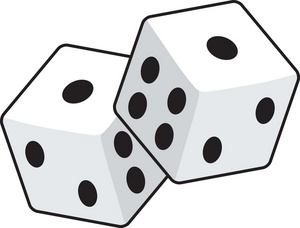
\includegraphics[width=0.3\textwidth]{dice.png}
\clearpage
\end{titlepage}

\tableofcontents
\addcontentsline{toc}{section}{References}
\thispagestyle{empty}
\cleardoublepage
\setcounter{page}{1}

\section{Q1i: Simulation of Probability Distributions}
\subsection{Univariate System Model}
\subsection{Long Run Averages}
\subsection{Covariance}
\subsection{Condition Distribution of S3}
\clearpage

\newgeometry{top=1cm,left=1cm,bottom=2cm,right=1cm}
\section{Q1ii: Probability Distributions}
\subsection{Probability Distribution}
Three dice can be rolled in a variety of 216 ways (6*6*6) over a probability distribution shown below. The possible combinations for each die results in varied probabilities for each number, where a greater number of combinations results in a higher probabilistic outcome, and thus over the long run, results in a variance of probabilities for each dice combination. The probability of each number rolled tends from the value of the number of combinations that can be possibly formed for that combination, with respect to the total number of combinations possible for n dice.
\begin{table}[h]
\centering
\begin{tabular}{llllllll}
Sum & \multicolumn{5}{l}{Dice Combinations}  & Combinations & Probability \\
3            & 1,1,1 &        &       &       &       & 1                  & 0.005       \\
4            & 1,1,2 &        &       &       &       & 3                  & 0.014       \\
5            & 1,2,2 & 1,1,3  &       &       &       & 6                  & 0.028       \\
6            & 1,1,4 & 1,2,3  & 2,2,2 &       &       & 10                 & 0.046       \\
7            & 1,1,5 & 1,2,4  & 1,3,3 & 2,2,3 &       & 15                 & 0.069       \\
8            & 1,1,6 & 1,2,5  & 1,3,4 & 2,2,4 &       & 21                 & 0.097       \\
9            & 1,3,5 & 1,4,4  & 1,2,6 & 2,2,5 & 3,3,3 & 25                 & 0.116       \\
10           & 1,3,6 & 1,4,5  & 2,2,6 & 2,3,5 & 3,3,4 & 27                 & 0.125       \\
11           & 1,4,6 & 1,5,5  & 2,3,6 & 2,4,5 & 3,4,4 & 27                 & 0.125       \\
12           & 1,5,6 & 2,4,6, & 2,2,5 & 3,3,6 & 4,4,4 & 25                 & 0.116       \\
13           & 1,6,6 & 2,5,6  & 3,5,5 & 3,4,6 &       & 21                 & 0.097       \\
14           & 2,6,6 & 3,5,6  & 4,4,6 & 4,5,5 &       & 15                 & 0.069       \\
15           & 3,6,6 & 4,5,6  & 5,5,5 &       &       & 10                 & 0.046       \\
16           & 4,6,6 & 5,5,6  &       &       &       & 6                  & 0.028       \\
17           & 5,6,6 &        &       &       &       & 3                  & 0.014       \\
18           & 6,6,6 &        &       &       &       & 1                  & 0.005       \\
             &       &        &       &       &       & 216                & 1          
\end{tabular}
\caption{Probability Distribution of Combinations}
\end{table}
\subsection{Multinomial Theorem}
The multinomial theorem is a \emph{generating function} by which a probability distribution of dice sums may be calculated and expressed. The series is defined by the power of the number, where the exponent itself is a polynomial with respect to the number rolled by the die for any positive integer m and non-negative integer n.
$$(x_1+x_2+...+x_m)^n=\sum_{k_1+k_2+...+k_m=n}{}\frac{n!}{k_1!k_2!...k_m!}\prod_{1\leq t\leq m}^{}x_{t}^{k_t}$$
In the case of $S_n$ where n dice of 6 sides have been rolled
$$G(S_n)=\left(\sum_{k=1}^{6}x^k\right)^n=(x^1+x^2+x^3+x^4+x^5+x^6)^n$$
Such that for multiple dice
\begin{align*}
G(S_1)&=x^1+x^2+x^3+x^4+x^5+x^6\\
G(S_2)&=(x^1+x^2+x^3+x^4+x^5+x^6)^2\\
&=x^2+2x^3+3x^4+4x^5+5x^6+6x^7+5x^8+4x^9+3x^{10}+2x^{11}+x^{12}
\end{align*}

\subsection{Expected Value and Variance}
Expected value is defined as the product of given value with respect to the probabilistic outcome of that value, as a summation of all the possible values  within that set for a randomly distributed variable X:
\begin{align*}
E[X_n]=x_np_n \quad \textrm{where} \quad E[X]=\sum_{i=1}^{n}x_np_n
\end{align*}
Given the probability distribution, the expected value is calculated as such:
$$E[X_1]=1*\frac{1}{6}+1*\frac{2}{6}+1*\frac{3}{6}+1*\frac{4}{6}+1*\frac{5}{6}+1*\frac{6}{6}=3.5$$
In the case of having three dice, this method can be extended to encapsulate a wider range of values over two additional dice:
$$E[X_3]=3*\frac{1}{216}+4*\frac{3}{216}+5*\frac{6}{216}+6*\frac{10}{216}+7*\frac{15}{216}+8*\frac{21}{216}+9*\frac{25}{216}+10*\frac{27}{216}+$$
$$11*\frac{27}{216}+12*\frac{25}{216}+13*\frac{21}{216}+14*\frac{15}{216}+15*\frac{10}{216}+16*\frac{6}{216}+17*\frac{3}{216}+18*\frac{1}{216}$$\\
The rolling of dice in such a way is denoted as an independent event, as the dice rolls in the future are not dependent on previous rolls and do not affect the outcome of values, where essentially the expected outcome of the event is given by:
$$E[X+Y+Z]=E[X]+E[Y]+E[Z]$$
Given the independence of each die roll, the expected value for three rolls is given by:
$$E[X+Y+Z]=3.5+3.5+3.5=10.5$$
Thus confirming the supposition by applying probabilistic arguments to the real-world. Ergo, variance of a random variable is denoted by the following:
\begin{align*}
\sigma^2(X)&=E[(X-\mu)^2]\\
&=E[X^2-2XE[X]+E(X)^2]\\
&=E[X^2]-2E[X]E[X]+(E[X])^2\\
&=E[X^2]-(E[X])^2
\end{align*}
Therefore the variance for the set can be determined from the above equations results in the following using the square of the value rolled from 1-6 a total of 1 time:
$$E[X_1^2]=1*\frac{1}{6}+4*\frac{1}{6}+9*\frac{1}{6}+16*\frac{1}{6}+25*\frac{1}{6}+36*\frac{1}{6}=15.16$$
$$\sigma^2(X_1)=15.16-(3.5)^2=2.91$$
Given the joint probabilities via S3, S4, M3 and N4; the expected value of M3 is the sum-product of the marginal probability of M3. The same is true for the expected value of M4 with respect to M4 itself. Thus,
$$E[M_3]=0.005+0.065+0.264+0.630+1.481+2.529=4.972$$
Similar to one die, calculating the sum of three dice results in a similar manner:
\begin{align*}
E[X_3^2]&=9*\frac{1}{216}+16*\frac{3}{216}+49*\frac{6}{216}+64*\frac{10}{216}+81*\frac{15}{216}+100*\frac{21}{216}\\&+121*\frac{27}{216}+144*\frac{27}{216}+169*\frac{21}{216}+196*\frac{15}{216}+225*\frac{10}{216}\\&+256*\frac{6}{216}+289*\frac{3}{216}+324*\frac{1}{216} = 119\\
\sigma^2(X_3)&=119-(10.5^2)=8.75
\end{align*}
For each given roll, there is independence between variables. Therefore the total variance is the sum of the individual variances within the set:
\begin{align*}
\sigma^2(S_3)&=\sigma^2(X_1)+\sigma^2(X_2)+\sigma^2(X_3)\\
&=2.91+2.91+2.91=8.73\approx8.75
\end{align*}
\begin{align*}
\centering
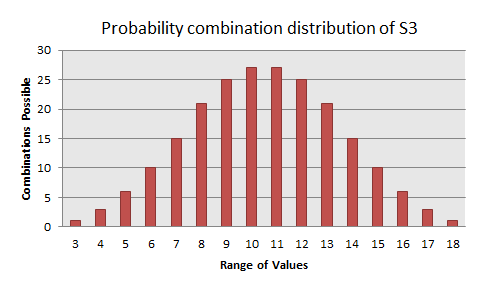
\includegraphics[width=0.5\textwidth]{PD_S3.png}
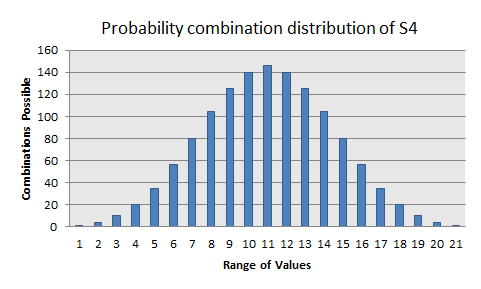
\includegraphics[width=0.5\textwidth]{PD_S4.png}
\end{align*}
\subsection{Covariance}
Covariance in a dataset is a measure of how much two random variables change together within a given time. Covariance within the data sets may be defined as followed
\begin{align*}
\sigma(X,Y)&=E[(X-E(X))(Y-E(Y))]\\
&=E[XY-XE(Y)-Y(EX)+E(X)E(Y)]\\
&=E(XY)-E(X)E(Y)-E(Y)E(X)+E(X)E(Y)\\
&=E(XY)-E(X)E(Y)
\end{align*}
Thus calculating $\sigma(S_3,M_3)$ for the joint probabilities of $(S_3,M_3)$ and $(S_4,M_4)$ respectively gives
\begin{align*}
\sigma(S_3,M_3)&=54.764-(4.972*(3*3.5))=2.558\\
\sigma(S_4,M_4)&=74.589-(5.181*(4*3.5))=2.055
\end{align*}

\subsection{Long Run Expected Values and Variances}
Following the \emph{Central Limit Theorem} which implies that $X_1,X_2,...,X_n$ are all independent random variables, where each random variable within the set pertains to tending to the same expected value, $\mu$, and standard deviation, $\sigma^2$, within the distribution given that the population is sufficiently large with n values of dice summation.
\begin{align*}
\centering
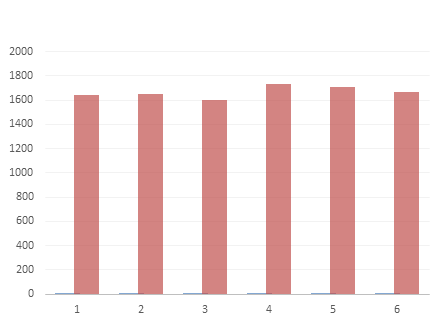
\includegraphics[width=0.5\textwidth]{s1.png}
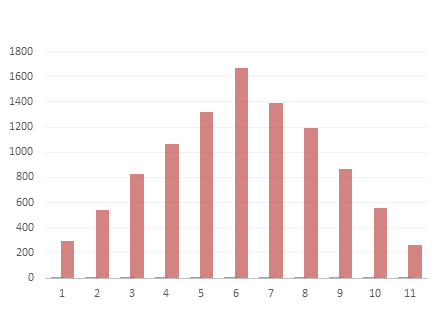
\includegraphics[width=0.5\textwidth]{s2.png}
\end{align*}
\begin{align*}
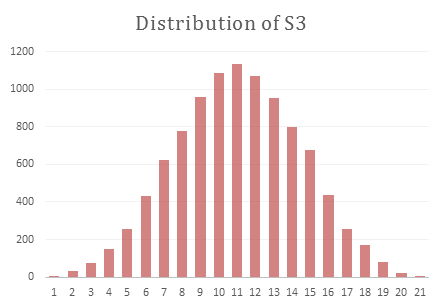
\includegraphics[width=0.5\textwidth]{s3.png}
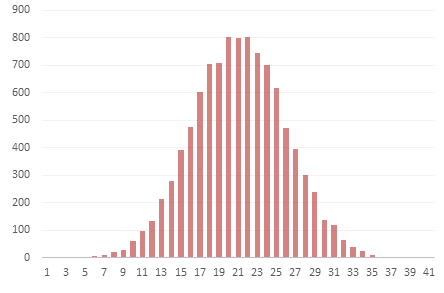
\includegraphics[width=0.5\textwidth]{s4.png}
\end{align*}
The above charts are $S_1$, $S_2$, $S_4$, and $S_8$ which demonstrate the effects of tending to the normal distribution curve as n samples approaches infinity.  Ergo, the expected value of $E[S_k]$ is therefore shown to be $E[S_k]=K*E[S_1]$, while the expected long run variance $V[S_k]$ is shown to be $V[S_k]=K*V[S_k]$
\section{Q1iii: Law of Large Numbers}
\subsection{Converging}
There are various versions for The Law of Large Numbers that basically all mean the same thing. As the sample size grows indefinitely, the mean value of the data will converge to the “expected value” for the data.
The Weak Law states that as n approaches infinity, for all $\epsilon > 0$, the probability of $|\bar{X}\bar{n} - \mu|> \epsilon$ is 0, whilst the \emph{Strong Law} states that for some large number N; $n>N$, the probability of $\bar{X}\bar{n} = \mu$ is 1. The key difference between them is that the Weak Law leaves open the possibility of an infinite number of tests before convergence but the Strong Law states that convergence is achieved for all large enough $n$. Borel also investigated this phenomenon and produced his own \emph{Law of Large Numbers}:\\
For an experiment repeated independently under identical conditions, the ratio of occurrence of any specified event approximately equals the probability of the event's occurrence on any trial if it is repeated a large enough number of times.
\\
From looking at section 2.3 we see that $E[S_1] = 3.5$ and it is given that $E[S_k]=k[E[S_1]]$ (see section 2.5). This means that:
\\\\
\begin{minipage}{0.5\textwidth}
\begin{flushleft} 
$$E[S_3]=3[E[S_1]]=10.5$$
\end{flushleft}
\end{minipage}
~
\begin{minipage}{0.5\textwidth}
\begin{flushleft} 
$$E[S_4]=4[E[S_1]]=14$$
\end{flushleft}
\end{minipage}
\\\\
From looking at the graphs in section 1.2 it is clear that the Average Value of S3, after initially fluctuating from the expected value, begins to converge to 10.5. We see a similar occurrence regarding the Average value of $S_4$ converging to 14. Those graphs clearly illustrate the Law of Large Numbers.
\\
What is evident is the importance of running many simulations as even after 150 trials the average value of $S_3$ is fluctuating back and forth around 10, as opposed to near the expected value of 10.5. A similar problem can be observed with regards to $S_4$. Clearly the initial skew is due to a high value within the first few trials. As you can then see, this is eventually cancelled out with many trials and the overall mean value will converge upon the expected value. The key word is that it “eventually”, not “immediately”, converges to the expected value. It is this misinterpretation that leads to flawed gambling strategies, such as \emph{Martingale strategy} for the roulette wheel which will be analysed in section 4.

\section{Q2: Martingale-Roulette Investigation}
\subsection{Martingale Strategies}
Roulette is a casino game of French origin that has become a staple game found in the majority of casinos worldwide. Roulette’s popularity is due to the fact that it involves no player skill whatsoever, making it the go-to game of casino “newbies”. However this comes with a price, the casino holds a great edge in every spin of the wheel. For this project I will focus on the European version of Roulette which holds a lesser house edge than that of American Roulette, due to the presence of only 1 zero in European Roulette compared to the 2 zeros of American Roulette.
\subsection{Payoff}
\begin{table}[h]
\centering
\begin{tabular}{cccc}
\begin{tabular}[c]{@{}c@{}}European Roulette\\ House Edge\end{tabular} & \begin{tabular}[c]{@{}c@{}}House Edge Calculation\\ $P(loss)*(stake$ $lost)+P(win)*return$ \end{tabular} & \begin{tabular}[c]{@{}c@{}}Percentage\\ House Edge\end{tabular} & \begin{tabular}[c]{@{}c@{}}Expected Value\\ on \$10 Bet\end{tabular} \\
Single \# Betting                                                      & $\frac{36}{37}*(-1)+\frac{1}{37}*(35)$                                            & -2.70\%                                                         & -\$0.27                                                              \\
Outside Betting                                                        & $\frac{19}{37}*(-1)+\frac{18}{37}*(1)$                                  & -2.70\%                                                         & -\$0.27                                                             
\end{tabular}
\caption{Martingale Strategy Applied to Roulette}
\end{table}
As you can see this is a very foreboding prospect for gamblers as they are expected to lose money on every bet they place. Naturally gamblers will want to try and offset this house edge and the most common way of attempting to do this is through the use of betting systems to maximise their winnings or minimise their losses. As convincing as many of these betting systems appear to be, none of them can change the edge of the game being played.

One of the most well-known betting strategies is the “Martingale” betting system. Martingale originated in $18^{th}$ century France where roulette was very popular at the time. Martingale involves betting on even money bets usually in roulette (Red or Black, odd or even) or craps (pass/come bets). After every loss the player doubles their bet until they win, in which case they return to their base unit bet. The idea behind Martingale is that no matter how many times the player loses, a win will net them a profit equal to their base bet. However there are two key problems facing a player that utilizes the Martingale Strategy.

\begin{enumerate}
\item Martingale can only be completely effective if the player has infinite money as a long run of losses will leave the player betting astronomical amounts of money.
\item Casinos often have limits on the stakes that can be placed at any table. Then when the player runs on a streak of losses, they get to a point when the casino will not let them increase their bet any further, breaking the system.
\end{enumerate}

A simulation was carried out using the RANDBETWEEN() function to mimic the spin of the roulette wheel 1,000 times. This would equate to roughly 9 hours playing time for a gambler alone at a table.

To simplify the simulation, the bet chosen was odd or even as Excel has a useful modulo function, however we would see the same results had any other even money bet been used. A base unit bet of \$5 was used as this is often times the minimum bet accepted at a roulette table. A running count of net profit was calculated along with a tally of the streaks of wins and losses and the cumulative difference between wins and losses.

The downfall of Martingale can be seen clearly from the results of the simulation. While the strategy exhibits a returns profile that is deceptively low risk with steady returns, there are sometimes catastrophic sequences that will cause the gambler to run into ruin. At the lowest point on the Net Profit graph, the player was down \$9,535 requiring a bet of \$10,240 to return the player into profit. This is impossible to do in reality as the casinos will only allow a maximum bet of around \$2,000 on outside bets.

This is good example of a \emph{Taleb Distribution} or \emph{Taleb Payoff}. The gambler usually wins a small net reward causing the illusion of a sound strategy. However the gambler’s expected value still remains less than zero due to the inherent house edge in the game and the small probability that he will suffer catastrophic loss. The size of the bet increases exponentially and this, combined with the fact that streaks of consecutive losses are more common than expected, can leave the gambler broke.

Given I walk into a casino with \$1,000 and proceed to employ Martingale starting at \$5, it would only take a streak of 7 losses in a row to cause me to be unable to bet enough on the $8^{th}$ bet to continue with the strategy.
$$\sum^{7}_{n=0}5(2^n)=\$1,275$$
The probability of 7 losses in a row when playing European Roulette is as follows:
$$\left(\frac{19}{37}\right)^7=0.00942$$
Although this is appears quite low, no player expects to walk into a casino and only bet one 1 spin of the roulette wheel. The more bets you place, the more likely the player is to go bankrupt however during the game the player does not see this. Instead the player sees steady returns of his unit bet multiple times per minute. This causes the player to continue betting and eventually run into ruin. Intuitively, we can look at the results of each bet on a game of roulette as a sequence of independent and identically distributed random variables. As expected value is a linear operator, we have:
$$E(b_1+b_2+...+b_n)=E(b_1)+E(b_2)+...+E(b_n)$$
\subsection{Conclusion}
As the bets are independent in roulette, the expected value of any bet does not rely on any previous bet. As we have calculated at the start of the question, roulette holds an inherent negative expected value on every bet. Therefore our expected value will always be negative as the sum of negative numbers is always negative. From this we can conclude that there is no way to create a profitable betting strategy for roulette due to the independence of its outcomes. The best way to win at Roulette is to avoid playing in the first place.
\begin{thebibliography}{3}
\bibitem{kilbyj}
  Jim Kilby, Jim Fox, Anthony F. Lucas,
  \emph{Casino Operation Management, 2nd Edition},
  Wiley (2006).
\bibitem{talebn}
  Nassim Nicholas Taleb,
  \emph{Fooled by Randomness: The Hidden Role of Chance in Life and in the Markets},
  Random House Trade (2005).
\bibitem{tijmsh}
  Henk Tijms,
  \emph{Understanding Probability, 3rd Edition},
  Cambridge University Press (2012).
\end{thebibliography}
\end{document}
